% Copyright 2009 by Tomasz Mazur
%
% This file may be distributed and/or modified in all ways.


\documentclass[xcolor=pdftex,t,11pt]{beamer}

%%%%%%%%%%%%%%%%%%%%%%%%%%%%%%%%%%
%       SET OPTIONS BELOW        %
%%%%%%%%%%%%%%%%%%%%%%%%%%%%%%%%%%

\usetheme[
% Toggle showing page counter
pagecounter=true,
%
% String to be used between the current page and the
% total page count, e.g. of, /, from, etc.
pageofpages=of,
%
% Defines the shape of bullet points. Available options: circle, square
bullet=circle,
%
% Show a line below the frame title. 
titleline=true,
%
% Set the style of the title page (true for fancy, false for standard)
alternativetitlepage=true,
%
% Institution logo for fancy title page.
% Comment out to remove the logo from the title page.
% IMPORTANT: THERE IS A BUG IN SOME VERSIONS OF PDFLATEX AND FONTS
% ON THE LOGOS ARE NOT RENDERED PROPERLY. IN SUCH A CASE ADD `2` 
% TO THE NAME OF THE LOGO, E.G. comlab2 INSTEAD OF comlab
%titlepagelogo=images/titlepage/ou,
%
% Department footer logo for fancy title page
% Comment out to remove the logo from the footer of the title page/
% IMPORTANT: THERE IS A BUG IN SOME VERSIONS OF PDFLATEX AND FONTS
% ON THE LOGOS ARE NOT RENDERED PROPERLY. IN SUCH A CASE ADD `2` 
% TO THE NAME OF THE LOGO, E.G. comlab2 INSTEAD OF comlab
%titlepagefooterlogo=images/titlepage/comlab,
%
% Institution/department logo for ordinary slides
% Comment this line out to remove the logo from all the pages.
% Available logos are: ou, comlab, comlabinline, comlabou
% IMPORTANT: THERE IS A BUG IN SOME VERSIONS OF PDFLATEX AND FONTS
% ON THE LOGOS ARE NOT RENDERED PROPERLY. IN SUCH A CASE ADD `2` 
% TO THE NAME OF THE LOGO, E.G. comlab2 INSTEAD OF comlab
%ordinarypageslogo=TU-Signet,
%
%
% Add watermark in the bottom right corner
%watermark=<filename>,
%
% Set the height of the watermark.
%watermarkheight=100pt,
%
% The watermark image is 4 times bigger than watermarkheight.
%watermarkheightmult=4,
]{Torino}

% Select color theme. Available options are:
% mininmal, greenandblue, blue, red
\usecolortheme{blue}

%Select different font themes.Available options are:
% default, serif, structurebold, structureitalicserif, structuresmallcapsserif
\usefonttheme{structurebold}

\usepackage{tikz}
\usepackage{pgf}

\pgfdeclareimage[height=6ex]{ou-logo}{images/ou}

\logo{\pgfuseimage{ou-logo}}

\usepackage{listings}

\lstset{language=C,
 basicstyle=\tiny
 }

\usepackage{ifthen}

\usepackage{moreverb}
\usepackage{pgf}
\usepackage{tikz}
\usetikzlibrary{arrows, automata, shapes.multipart, chains, positioning, fit}

\usepackage{pifont}
\newcommand{\xmark}{\ding{55}}

\usepackage{color}
\definecolor{light-gray}{gray}{0.80}


\newcommand{\hpathlen}{\ensuremath{\mathit{pathLength}}\xspace}
\newcommand{\halloc}{\ensuremath{\mathit{new}}\xspace}
\newcommand{\hassign}{\ensuremath{\mathit{assign}}\xspace}
\newcommand{\hlookup}{\ensuremath{\mathit{lookup}}\xspace}
\newcommand{\hupdate}{\ensuremath{\mathit{update}}\xspace}
\newcommand{\halias}{\ensuremath{\mathit{alias}}\xspace}
\newcommand{\hisnull}{\ensuremath{\mathit{isNull}}\xspace}
\newcommand{\hispath}{\ensuremath{\mathit{isPath}}\xspace}
\newcommand{\hcircular}{\ensuremath{\mathit{circular}}\xspace}
%\newcommand{\id}{\ensuremath{\mathrm{id}}\xspace}
\newcommand{\hsubdivide}{\ensuremath{\mathit{subdivide}}\xspace}
\newcommand{\hfresh}{\ensuremath{\mathit{fresh}()}\xspace}

\newcommand{\defeq}{\ensuremath{\stackrel{\mathrm{def}}{=}}}

\newcommand{\kalashnikov}{{\sc Kalashnikov}\xspace}
\newcommand{\shakira}{{\sc Shakira}\xspace}


%%%%%%%%%%%%%%%%%%%%%%%%%%%%%%%%%%
%       PRESENTATION INFO        %
%%%%%%%%%%%%%%%%%%%%%%%%%%%%%%%%%%

\author{Cristina David \and Daniel Kroening \and Matt Lewis}
\title{Precise, Second-Order Verification}
%\subtitle{}
\institute{Oxford University}
\date{\today}

\begin{document}



%%%%%%%%%%%%%%%%%%%%%%%%%%%%%%%%%%
%       SLIDE DEFINITIONS        %
%%%%%%%%%%%%%%%%%%%%%%%%%%%%%%%%%%

\begin{frame}[plain]
  \titlepage
\end{frame}

\iffalse
\begin{frame}{Outline}
  \tableofcontents
\end{frame}
\fi

\section{Motivation}


\begin{frame}[fragile]{Motivation}
Does this program terminate?
\begin{center}
\begin{minipage}{0.4\linewidth}
 \begin{lstlisting}[language=C,basicstyle=\normalsize]
while (x > 0) {
  x++;
}
 \end{lstlisting}
\end{minipage}
\end{center}

\pause

That depends...

It \emph{does not} terminate if the program operates on integers...

But it \emph{does} terminate if the program operates on fixed-width words
(-x decreases monotonically and is bounded by -MAXINT).

\end{frame}

\begin{frame}[fragile]{Motivation}
Which of these guys terminates?
\begin{center}
\begin{minipage}{0.45\linewidth}
 \begin{lstlisting}[language=C,basicstyle=\normalsize]
while (x > 0) {
  x = (x - 1) & x;
}
\end{lstlisting}
\end{minipage}
\begin{minipage}{0.45\linewidth}
 \begin{lstlisting}[language=C,basicstyle=\normalsize]
while (x > 0) {
  x = (x + 1) & x;
}
\end{lstlisting}
\end{minipage}
\end{center}

\pause

The left one does (x decreases monotonically), but the right one doesn't ($2 \rightarrow 2 \rightarrow \dots$).
\end{frame}

\begin{frame}{Motivation}
Proving program termination has been a big deal for a while.

It'd be nice if we could automatically prove termination for programs that run on computers.
\end{frame}

\section{Proving Termination}
\begin{frame}{What Does a Termination Proof Look Like?}
We prove that a program terminates by finding a \emph{ranking function}.

\vspace{1em}

If we have a transition relation $T$ and a loop guard $g$, a ranking function $R$
must meet the following criteria:
\begin{align}
 \forall x, x' \cdot & g(x) \Rightarrow R(x) > 0 ~ \wedge \\
                     & T(x, x') \Rightarrow R(x) > R(x')
\end{align}

Or more generally, $R$ must be an order-homomorphism with a well-founded co-domain (aka an ordinal).

\vspace{1em}

We are therefore in the business of finding ranking functions.
\end{frame}

\begin{frame}{Finding Ranking Functions}
Traditionally, people find ranking functions under some assumptions:

\begin{itemize}
 \item Programs are linear
 \item Ranking functions are linear
 \item Program variables are rationals
\end{itemize}

\vspace{1em}

With these assumptions in hand, one can deploy a very powerful piece of linear algebra: \emph{Farkas's lemma}.

This lemma makes light work of a ton of termination problems.

\vspace{1em}

But it's not for us.
\end{frame}


\begin{frame}{Synthesing Ranking Functions}
Our approach is to use \emph{program synthesis} to generate ranking functions.

\vspace{1em}

We're going to set up a program synthesis problem that will allow us to solve
the following 2nd-order satisfaction problem:
\begin{align*}
 \exists R . \forall x, x' \cdot & g(x) \Rightarrow R(x) > 0 ~ \wedge \\
                             & T(x, x') \Rightarrow R(x) > R(x')
\end{align*}

\pause

\vspace{1em}

In other words: ``Is there a ranking function for my program?''

\end{frame}

\begin{frame}{Specifying a Ranking Function}
Our program synthesiser needs a \emph{specification}, which takes the form of a C function.

\vspace{1em}

The specification function takes two arguments: a candidate program $P$ and an input $x$.
If $P$ gives the correct output when fed $x$, our specification function returns true,
otherwise it returns false.
\end{frame}

\begin{frame}[fragile]{A Specification}

\vspace{-1em}

\begin{center}
\begin{minipage}{.6\textwidth}
\begin{lstlisting}[language=C++,basicstyle=\small]
bool spec(prog_t *p, int x) {
  int y = exec(p, x);

  if (y >= x)
    return true;
  else
    return false;
}
\end{lstlisting}
\end{minipage}
\end{center}

\pause

Two of the possible programs:

\begin{itemize}
  \item[] \texttt{int f(int x) \{ return x; \}} 
  \item[] \texttt{int f(int x) \{ return MAXINT; \}}
\end{itemize}

\end{frame}

\begin{frame}[fragile]{Specifying a Ranking Function}
\vspace{-1em}

\begin{center}
\begin{minipage}{0.6\textwidth}
\begin{lstlisting}[language=c++,basicstyle=\small]
int spec(prog_t *p, int x) {
  int r1 = exec(p, x);

  if (g(x)) {
    if (r1 <= 0)
      return false;

    int y = body(x);
    int r2 = exec(p, y);
    
    if (r1 <= r2)
      return false;
  }
  
  return true;
}
\end{lstlisting}
\end{minipage}
\end{center}
\end{frame}

\iffalse

\section{Abstract Program Synthesis}
\begin{frame}{The Synthesis Formula}
Our high-level goal is to synthesise programs that meet some specification.

\pause

Abstractly, a program $P$ computes some function from an input set $I$ to an output set $O$:
$$P : I \rightarrow O$$

\pause

A specification is a relation between inputs and outputs:
$$\sigma \subseteq I \times O$$

\pause

The synthesis problem is to find a program that meets the specification on all inputs:
$$\exists P . \forall x \in I . \sigma(x, P(x))$$
\end{frame}
\fi

\begin{frame}[fragile]{Solving the Synthesis Formula with CEGIS}
 Solving second order formulae is hard.  Instead we'll alternately solve two \emph{first-order} formulae
 in a refinement loop:

 \vspace{1cm}
 
  \begin{tikzpicture}[->,>=stealth',shorten >=1pt,auto,
 semithick, initial text=]

  \matrix[nodes={draw, fill=none, scale=1, shape=rectangle, minimum height=1cm, minimum width=1.5cm},
          row sep=2cm, column sep=3cm] {
   \node (synth) {Synthesise};
   &
   \node (verif) {Verify}; %\\
   %\node[draw=none] {};
   &
   \node[ellipse] (done) {Done}; \\
  };

   \path
    (synth) edge [bend left] node {Candidate program} (verif)
    (verif) edge [bend left] node {Counterexample input} (synth)
    (verif) edge node {Valid} (done);
 \end{tikzpicture}
\end{frame}

\begin{frame}{First-order Synthesis}
 If we have some small set of test inputs $\{ x_0, \dots, x_N\}$, we can find a program that is correct on just that set:

 $$\exists P . \sigma(x_0, P(x_0)) \wedge \dots \wedge \sigma(x_N, P(x_N))$$
\end{frame}

\begin{frame}{First-order Verification}
 If we have some program $P$ that might be correct, we can check whether it is in fact correct:
 
 $$\exists x . \lnot \sigma(x, P(x))$$
 
 If this formula is \emph{satisfiable}, $P$ is \emph{not} correct and we have found an input on which it is incorrect.
 We can add this input to our set of test inputs and loop back to synthesising a new program.
\end{frame}

\section{Program Synthesis}
\iffalse
\begin{frame}{Concrete Synthesis in C}
 We're using C as an implementation language.  To do that we need:
 
 \begin{itemize}
  \item A way of encoding programs as \emph{finite structures} in C.
  \item A way of encoding the first-order synthesis and verification formulae in C.
  \item A way of checking properties of C programs.
 \end{itemize}
\end{frame}

\begin{frame}[fragile]{Encoding Programs in C}
 To encode the programs we will synthesise, we just make a very simple language and an interpreter for it.  Programs
 in our language look like this:

 \vspace{0.7cm}

\begin{center}
\begin{minipage}{0.3\linewidth}
\begin{verbatimtab}
t1 = neg x
t2 = add t1 1
return t2
\end{verbatimtab}
\end{minipage}
\end{center}

\end{frame}

\fi

\begin{frame}{Complexity}
By far the dominant factor in how long synthesis takes is the length of the shortest correct program.

\vspace{1em}

This is called the \emph{Kolmogorov complexity} of the function being computed.

\vspace{1em}

For termination, this gives us the property that our runtime doesn't depend very heavily
on the size of the program we are analysing.  It is instead almost entirely determined by the
size of the shortest program that computes a valid ranking function.
\end{frame}


\begin{frame}{Genetic Programming}
The flip side of being so dominated by Kolmogorov complexity is that we
get \emph{really slow} beyond about 4 instructions.

\vspace{1em}

It turns out that \emph{genetic programming} helps a lot beyond this threshold.
\end{frame}

\begin{frame}{Genetic Programming}
Genetic programming is an evolutionary search strategy, which aims to find a program
that is ``fit'' according to some metric.

\vspace{1em}

It begins by generating a population of random programs.  This population is subjected to
\emph{evolution} over a period of many generations.

\vspace{1em}

At each generation, each individual's fitness is evaluated.  The fitter an individual is,
the greater its chance of breeding.

When two programs breed, their code is combined in some way (the crossover operation) and
the resulting child may be randomly modified (the mutation operator).  This child is copied
into the next generation.
\end{frame}

\begin{frame}{Genetic Programming Synthesis}
To use genetic programming for synthesis, we need to fix a useful fitness metric.

\vspace{1em}

For our purposes, we say that if a program meets the specification on $n$ test vectors, its
fitness is $n$.

Whenever we add a new test vector, we continue genetic programming with the most recent population
(the one that produced the most recent candidate program).  This is called \emph{incremental evolution}
and gives us a big speedup.

\vspace{1em}

Once we've found a program that passes all the tests, we return it and continue round the CEGIS
loop.
\end{frame}

\begin{frame}[fragile]{Oh, And One More Thing}
Does this terminate?  If so, what's the ranking function?

\begin{lstlisting}[basicstyle=\normalsize]
while (x > 0 && y > 0 && z > 0) {
  if (y > x) {
    y = z;
    x = nondet();
    z = x - 1;
  } else {
    z = z - 1;
    x = nondet();
    y = x - 1;
  }
}
\end{lstlisting}
\end{frame}


\section{Advanced Topics}
\begin{frame}{Conditional Termination}

\begin{align*}
\exists I, R \cdot \forall x, x' \cdot & P(x, x') \Rightarrow & I(x') \\
                                       & I(x) \wedge g(x) \wedge T(x, x') \Rightarrow & R(x) > 0 ~ \wedge \\
                                       & & R(x) > R(x') ~ \wedge \\
                                       & & I(x')
\end{align*}
\end{frame}

\begin{frame}{Sequential Loops}
\begin{align*}
\exists I_1, I_2, R \cdot \forall x, x' \cdot & P(x, x') \Rightarrow & I_1(x') \\
                                              & I_1(x) \wedge g_1(x) \wedge T_1(x, x') \Rightarrow & I_1(x') \\
                                              & I_1(x) \wedge \lnot g_1(x) \Rightarrow & I_2(x) \\
					      & I_2(x) \wedge g_2(x) \wedge T_2(x, x') \Rightarrow & R(x) > 0 ~ \wedge \\
					      & & R(x) > R(x') ~ \wedge \\
					      & & I_2(x')
\end{align*}
\end{frame}


\begin{frame}{Some Combinatorics}
A terminating program corresponds to a \emph{labelled partial order} on $2^k$ states.

\vspace{.7em}

Counting partial orders on a finite set turns out to be very hard (it's an open problem!).  However, asymptotics are known:
\begin{align*}
 P_n & = \left(1 + O \left( \frac{1}{n} \right) \right) \left( \sum_{i=1}^n \sum_{j=1}^{n-1} \binom{n}{i} \binom{n-i}{j} (2^i - 1)^j (2^j - 1)^{n - i - j}\right) \\
     & \sim O\left( 2^k \right)
\end{align*}

\end{frame}

\begin{frame}{More Combinatorics}
Linear functions on bitvectors correspond to \emph{permutations} of the natural ordering on bitvectors.

\vspace{1em}

There are $2^{2k}$ linear functions (although only half of these permute the full space, cf. generators of the group $2^k$).

\vspace{1em}

Each of these functions can show that each of the \emph{unlabelled} partial orders terminates.

The number of unlabelled partial orders over an $n$ element set is related to the number of labelled partial orders as:

$$p_n \sim {P_n \over n!}$$
\end{frame}

\begin{frame}{The Combinatorial Payoff}
Since there are $P_n$ terminating functions, and each of the $n^2$ linear functions can prove that
$p_n \sim {P_n \over n!}$ functions terminate, we can compute the probability that a random terminating
function can be proved to terminate with a linear argument:

$${2^k \times 2^k \over {2^k}!} \sim {1 \over {2^k}!}$$

\pause

\vspace{1em}

This number is very small, which to some degree justifies our aim of moving beyond linear ranking functions.

\end{frame}

\begin{frame}[fragile]{Heap}
 \centering
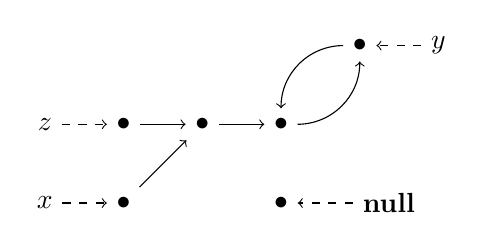
\begin{tikzpicture}
  %\node at (-.75,.25) {$h:$};

  \node (n1) {$\bullet$};
  \node (n2) [below of=n1] {$\bullet$};
  \node (n3) [right of=n1] {$\bullet$};
  \node (n4) [right of=n3] {$\bullet$};
  \node (n5) [right of=n4,above of=n4] {$\bullet$};
  \node (n6) [below of=n4] {$\bullet$};
  \node (x) [left of=n2] {$x$};
  \node (y) [right of=n5] {$y$};
  \node (z) [left  of=n1] {$z$};
  \node (null) [right=2em of n6] {\bf null};

  \path[draw,->] (n1) edge (n3)
		 (n2) edge (n3)
		 (n3) edge (n4)
		 (n4) edge[bend right=45] (n5)
		 (n5) edge[bend right=45] (n4);

  \path[dashed,->] (x) edge (n2)%
		   (y) edge (n5)%
		   (z) edge (n1)%
		   (null) edge (n6);
 \end{tikzpicture}
\end{frame}

\begin{frame}[fragile]{Heap Transformers}
 \centering
 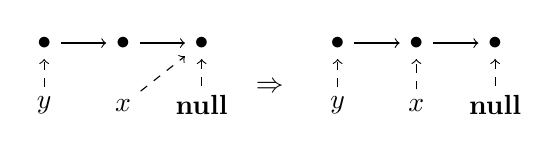
\begin{tikzpicture}
  \node (n1) {$\bullet$};
  \node [right of=n1] (n2) {$\bullet$};
  \node (n3) [right of=n2] {$\bullet$};

  \node (y) [below=1em of n1] {$y$};
  \node (x) [right of=y] {$x$};
  \node (null) [right of=x] {\bf null};

  \path[draw, ->] (n1) edge (n2) (n2) edge (n3);
  \path[dashed,->] (x) edge (n3) (y) edge (n1) (null) edge (n3);

  \node (mid) [below right = .5em and 1em of n3] {$\Rightarrow$};

  \node [above right = .5em and 1em of mid] (m1) {$\bullet$};
  \node (m2) [right of = m1] {$\bullet$};
  \node (m3) [right of = m2] {$\bullet$};

  \node (y) [below=1em of m1] {$y$};
  \node (x) [right of=y] {$x$};
  \node (null) [right of=x] {\bf null};

  \path[draw, ->] (m1) edge (m2) (m2) edge (m3);
  \path[dashed,->] (x) edge (m2) (y) edge (m1) (null) edge (m3);
 \end{tikzpicture}
 }

 \vfill
 $\hlookup(h, x, y)$ \\
 $x = y{\rightarrow}next;$
\end{frame}


\begin{frame}[fragile]{Fin}

\begin{center}
\includegraphics[width=.7\textwidth]{sloth.jpg}

\Huge
 Thank you!
\end{center}

\end{frame}


\end{document}